\section{Analisi tecnica: funzionamento e debolezze sfruttate}
\label{sec:analisi-tecnica}

% Persone 2 e 3 — circa 1,6 pagine complessive, figure incluse.
\subsection{npm: dall'account compromesso alla dipendenza malevola}
% Persona 2 — circa 0,8 pagina.
\subsubsection{Phishing e abuso dell'autorità di pubblicazione}

La compromissione dell'account npm del manutentore iniziò con un'e-mail di
phishing inviata dall'indirizzo \texttt{support@npmjs.help}. Il messaggio
minacciava la sospensione dell'account se il destinatario non avesse effettuato
il login entro due giorni, creando urgenza. Il manutentore riferì di aver
seguito il collegamento dal telefono e inserito le credenziali; in seguito perse
l'accesso all'account. L'episodio mostra come l'attaccante abbia sfruttato
l'identità legittima del publisher per pubblicare aggiornamenti: non fu
necessario compromettere l'intero registro npm~\cite{aikido2025}.

\begin{figure}[H]
    \centering
    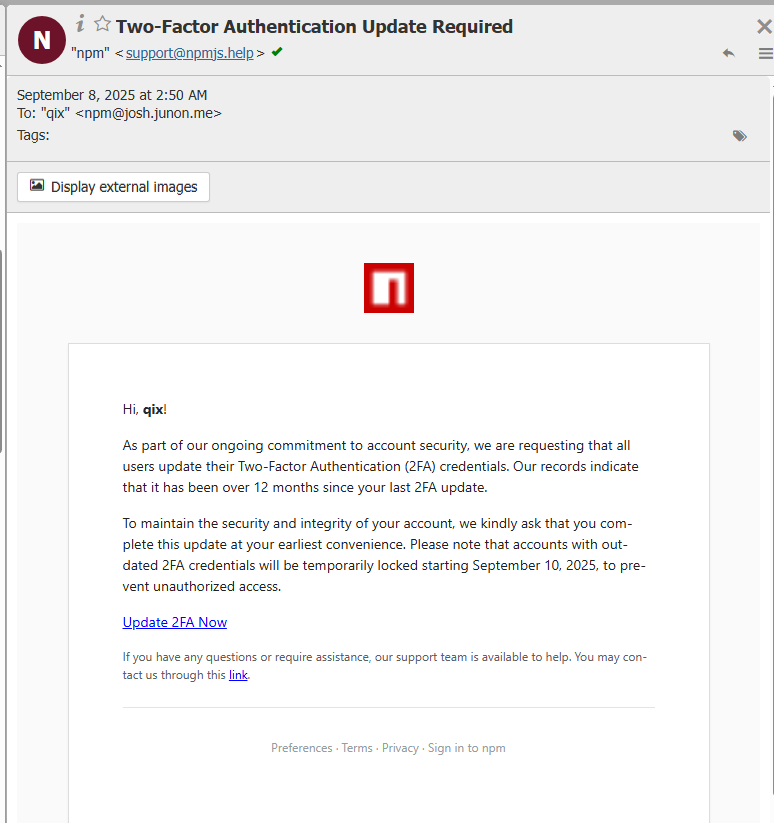
\includegraphics[width=0.68\textwidth]{mail_phishing.png}
    \caption{E-mail di phishing inviata al manutentore.}
    {\footnotesize Fonte: \cite{aikido2025}\par}
    \label{fig:phishing-npm}
\end{figure}

\subsubsection{Dalla pubblicazione malevola all'esecuzione nel browser}

Dopo aver ottenuto accesso all'account, l'attaccante pubblicò versioni
modificate di pacchetti mantenuti dalla vittima. Tra queste, \texttt{debug@4.4.2}
conservava le funzioni previste ma includeva codice JavaScript malevolo
~\cite{debug2025}. Il codice poteva raggiungere un'applicazione sia tramite
una dipendenza dichiarata direttamente, sia attraverso una dipendenza
transitiva. Se incluso nella build di un'applicazione web, il \emph{bundle}
(l'insieme di codice e dipendenze distribuito al browser) poteva portare il
codice fino agli utenti dell'applicazione. L'advisory del progetto specifica
che il comportamento malevolo riguardava l'ambiente browser; server e strumenti
da riga di comando non erano esposti a questo specifico comportamento
~\cite{debug2025,wiz2025}.

\begin{figure}[H]
    \centering
    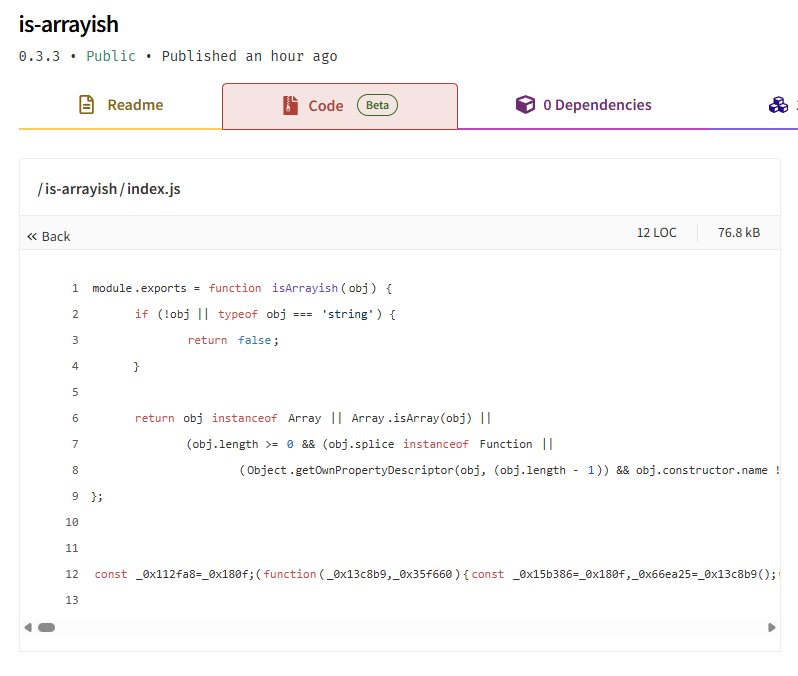
\includegraphics[width=0.9\textwidth]{Codice_malevolo.png}
    \caption{Esempio di codice malevolo nelle versioni compromesse.}
    {\footnotesize Fonte: \cite{aikido2025}\par}
    \label{fig:codice-malevolo-npm}
\end{figure}

\subsection{AUR: dalla modifica della ricetta all'esecuzione}
\label{subsec:aur-tecnica}
% Persona 3 — circa 0,8 pagina.
\subsubsection{Abuso della manutenzione della ricetta}
L'AUR ospita ricette \texttt{PKGBUILD} della comunità, non pacchetti binari
ufficiali; \texttt{makepkg} può recuperare file ed eseguire i comandi previsti
dalla ricetta~\cite{archwiki-aur,archwiki-makepkg}. Nel caso di
\texttt{gnome-\allowbreak randr-\allowbreak rust}, un nuovo manutentore
aggiunse uno script con
\texttt{npm install atomic-lockfile yargs}, senza una ragione tecnica
apparente. Un manutentore AUR confermò che la modifica era malevola e ripristinò
il commit precedente~\cite{aur-mail-gnome-randr}. Il punto abusato fu
l'adozione di una ricetta senza manutentore attivo, non l'accesso illegittimo
al registro npm o ai repository ufficiali di Arch.

Il pacchetto npm conteneva un hook \texttt{preinstall}, uno script eseguito
automaticamente durante l'installazione, che avviava un eseguibile Linux:
l'installazione della dipendenza trasferiva così l'esecuzione al payload
~\cite{aur-mail-gnome-randr}. Introdurre npm in un pacchetto AUR non è di per
sé malevolo, ma una dipendenza estranea al programma che esegue codice in fase
d'installazione è un'anomalia da verificare. La presenza di un altro gestore di
pacchetti, presa isolatamente, non prova quindi un attacco.

\subsubsection{Ambiente di esecuzione e privilegi}
La catena era: adozione della ricetta, modifica dello script \texttt{.install},
esecuzione di \texttt{npm install} nel callback \texttt{post\_install} e avvio
dell'hook \texttt{preinstall} del pacchetto npm
~\cite{aur-mail-gnome-randr}. La compilazione con \texttt{makepkg} e
l'installazione con \texttt{pacman} sono fasi distinte: Arch vieta di eseguire
\texttt{makepkg} come amministratore, mentre uno script \texttt{.install}
viene eseguito durante la transazione d'installazione o aggiornamento
~\cite{archwiki-makepkg,arch-alpm-scriptlet}. Se \texttt{pacman} è avviato
con privilegi elevati, il callback può ereditarli; ciò dipende comunque dalla
fase e dalla separazione dei privilegi adottata. Le fonti descrivono il
meccanismo, ma non quantificano installazioni o sistemi compromessi.
